\newpage
\section[Визуализация движения с потерей энергии]{Визуализация движения с потерей энергии}

Требуется визуализировать движение тела, брошенного под углом к горизонту с учетом <<отскока>>  от поверхности с потерей энергии.
Для упрощения модели потеря энергии при каждом соударении составляет 20\% от исходной.

Имеем уравнения движения тела в проекциях на оси:
\begin{equation*}
    \begin{aligned}
        &y(t) = y_{0} + v_{0y}t+\frac{a_{y}t^{2}}{2}; \\
        &x(t) = x_{0} + v_{0x}t+\frac{a_{x}t^{2}}{2}
    \end{aligned}
\end{equation*}

По второму закону Ньютона:
\begin{equation*}
    m\vec{a} = m\vec{g} \\
\end{equation*}

В проекциях на оси:
\begin{equation*}
    \begin{aligned}
        &Oy: \; ma_{y} = -mg; \;\; 
        a_{y} = -g; \\
        &Ox: \; ma_{x} = 0;
        a_{x} = 0
    \end{aligned}
\end{equation*}

Конечные уравнения движения тела:
\begin{equation*}
    \begin{aligned}
        &y(t) = y_{0} + v_{0y}t - \frac{gt^{2}}{2};\\
        &x(t) = x_{0} + v_{0x}t
    \end{aligned}
\end{equation*}

Конечная система дифференциальных уравнений:
\begin{equation*}
    \left\{
        \begin{aligned}
            &x(0) = 0 \\
            &x'(0) = v_{0} \\
            &x''(t) = 0
        \end{aligned}
    \right.; \;\;\;\;\;\;\;\;\;
    \left\{
        \begin{aligned}
            &y(0) = y_{0} \\
            &y'(0) = 0 \\
            &y''(t) = -g
        \end{aligned}
    \right. 
\end{equation*}

Дополнительное условие для моделирования <<отскока>>
при итеративном поиске численных решений дифференциальных уравнений:
\begin{equation*}
    y'(t) = 
    \left\{
        \begin{gathered}
            -0.9*y'(t), \;\; \text{если } y(t) = 0\\
            y'(t), \;\; \text{иначе} 
        \end{gathered}
    \right. 
\end{equation*}
\textit{Пояснение: при касании поверхности телом вертикальная скорость инвертируется с потерей 20\% (происходит <<отскок>> с потерей энергии)}

\newpage
Моделируем полет тела в Wolfram Mathematicа. 
Ипользуем инструменты: 
\textbf{NDSolve,} % (для численного решения систем дифференциальных уравнений), 
\textbf{Evaluate,} % (для интерполяции дискретных значений функций),
\textbf{ParametricPlot,} % (для построения графика параметрически заданной функции движения тела).\\[10pt]
\textbf{WhenEvent.}\\[10pt]

\textit{Листинг программы Matematica:}
\begin{figure}[ht]
    \begin{lstlisting}
(* Исходные параметры *)
g  = 9.8;
y0 = 10;
v0x = 0.5;

(* Получение численного решения систем дифференциальных уравнений *)
ndsY = NDSolve[
   {y''[t] == -g, y[0] == y0, y'[0] == 0, 
        WhenEvent[y[t] == 0, y'[t] -> -0.8 y'[t]]},
   y,
   {t, 0, 15}
];

ndsX = NDSolve[
   {x''[t] == 0, x[0] == 0, x'[0] == v0x},
   x,
   {t, 0, 15}
];

(* Построение графика *)
ParametricPlot[
 Evaluate[{x[t], y[t]} /. Flatten@{ndsX, ndsY}], 
 {t, 0, 12}
]
    \end{lstlisting} 
\end{figure}\\[0pt]
\textit{Полученный график:}
\begin{figure}[ht]
\centering
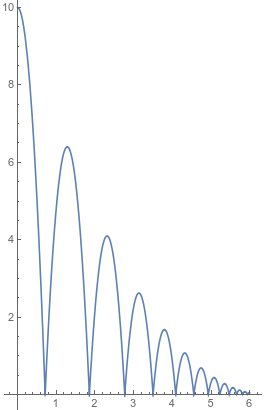
\includegraphics[width=5cm, height=5cm]{4-bounce.png}
\end{figure}
